\documentclass{article}

\usepackage{pdfpages}

\usepackage[hidelinks]{hyperref}

\usepackage{array}
\usepackage{tabularx}

\usepackage{comment}

\usepackage{tcolorbox}

\usepackage{graphicx}
\usepackage{subcaption}

\usepackage{amsmath}

\usepackage{float}

\usepackage[export]{adjustbox}

\usepackage[margin=1.25in]{geometry}

\newtcbox{\inlinecode}{on line, boxrule=0pt, boxsep=0pt, top=2pt, left=2pt, bottom=2pt, right=2pt, colback=gray!15, colframe=white, fontupper={\ttfamily \footnotesize}}

\begin{document}
\pagenumbering{gobble}

\includepdf[pages=-,scale=1,pagecommand={}]{cover-sheet.pdf}

\tableofcontents

\newpage
\pagenumbering{arabic}

\section{Executive Summary}
  \paragraph{}
  The goal of this project was to build a 4-bit shift register in Electric. A shift register is a digital device which can shift bits across a number of outputs. In our case, there are 4 outputs, Q0 through Q3. Every clock cycle, the value of the bit stored at Q2 is shifted to Q3, the value of Q1 is shifted to Q2, Q0 is shifted to Q1, and the state of input D is stored in Q0. This is a very useful circuit for a number of applications, as we can control four outputs with only two inputs: A clock pin and a data pin. Moreover, multiple shift registers can be chained together to create a larger shift register with more outputs. For example, I once worked on a project in which 8-bit shift registers were chained together to control 64 LEDs with just two pins on a microcontroller.

  \paragraph{}
  For this project, the shift register shifts data on the positive clock edge. This is done by making the shift register out of four positive-edge-triggered D flip-flops, each flip-flop representing one bit. The shift register also has a reset pin, which is active low. When the reset pin is pulled low, all four outputs are reset to logic low.

  \paragraph{}
  The project involves designing the shift register as both a schematic and a layout in Electric. Both the schematic and layout are simulated in LTspice and IRSIM to confirm that the shift register design works properly. Measurements are also taken using LTspice to determine the rise times, fall times, propagation delay, and power draw of the designs. For this project specifically, the layout is simulated with parasitic resistances and capacitances. This makes the simulation much more realistic, since more of the physical properties of the design are taken into account.

\section{Introduction and Background}
  \paragraph{}
  The design for the shift register consists of a couple of layers of designs. In order to build the shift register, we must first build a positive-edge-triggered master slave D flip-flop, and in order to build the flip-flop, we must first build a 2-input NAND gate and a 3-input NAND gate. The design for the positive-edge-triggered master-slave D flip-flop is shown in Figure \ref{fig:ff-design}. The design consists of two 2-input NAND gates and four 3-input NAND gates. The flip-flop has inputs for the clock signal, data signal, and reset line. It outputs Q and Q prime, however we will only be using Q for the shift register. The flip-flop works like a set of latches; while the clock is low, the "master" latch is set and the "slave" latch is held, and while the clock is high, the "master" latch is held while the "slave" latch is set. Because of this setup, the output of the flip-flop only changes to reflect the input on the positive clock edge. 


  \begin{figure}[H]
    \centering
    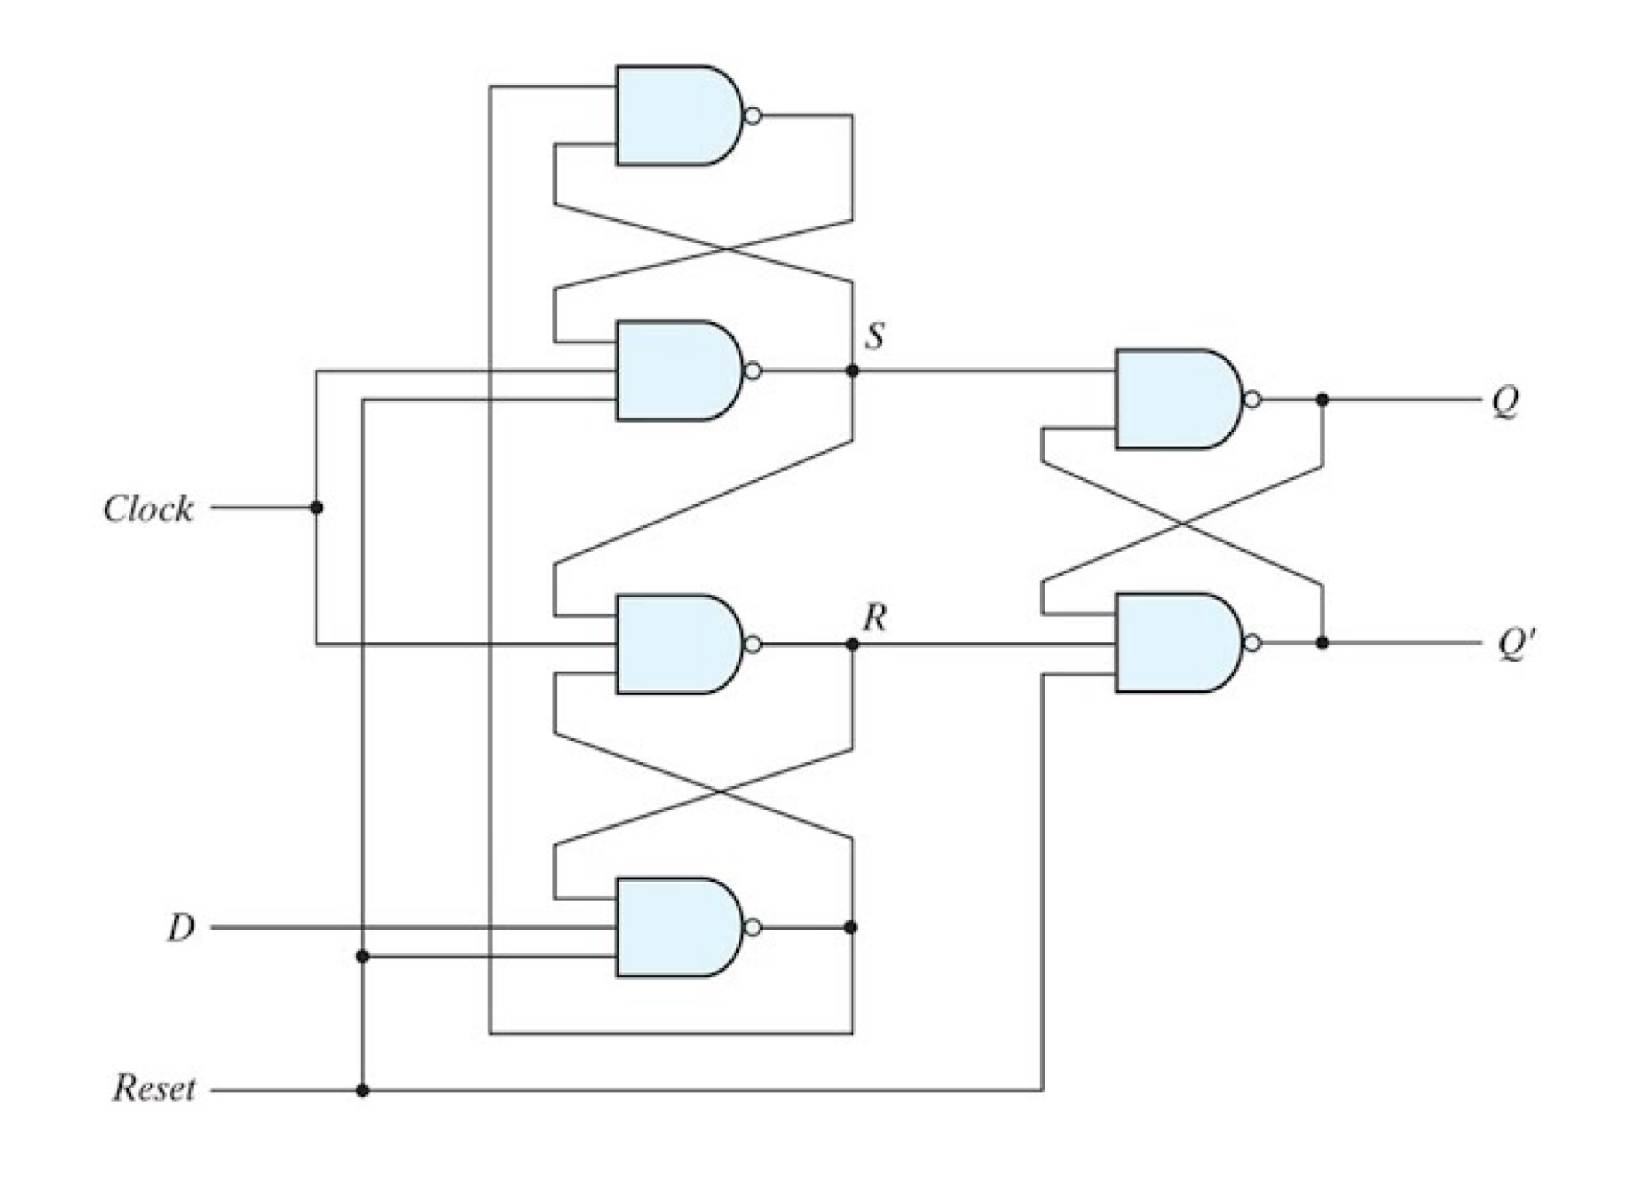
\includegraphics[width=0.7\linewidth, frame]{images/ff-design.png}
    \caption{The design for the positive-edge-triggered master-slave flip-flop.}
    \label{fig:ff-design}
  \end{figure}

  \paragraph{}
  Now that we understand how the flip-flop works, we can understand how the shift register works. As shown in Figure \ref{fig:shift-reg-design}, the 4-bit shift register is simply four positive-edge-triggered master-slave D flip-flops chained together. All of the reset pins of the flip-flops are connected together to create the reset line for the shift register. This reset line will reset all outputs to low when it is pulled low. The clock inputs are also tied together so that all of the flip-flops are triggered simultaneously at the positive clock-edge. The D input of the shift register is connected to the D input of the first flip-flop, and then the D input of each successive flip-flop is connected to the output of the previous flip-flop. This way, the data is shifted from left to right each positive clock edge.


  \begin{figure}[H]
    \centering
    \includegraphics[width=0.8\linewidth, frame]{images/shift-reg-design.png}
    \caption{The design for the 4-bit shift register consisting of four positive-edge-triggered master-slave D flip-flops.}
    \label{fig:shift-reg-design}
  \end{figure}

  \paragraph{}
  To give an example of how the shift register works, let us consider the following scenario. First, we pulse the reset pin low temporarily and then keep it high again. Now all outputs Q0, Q1, Q2, and Q3 are low. We will set D high for the first positive-edge of the clock. After the positive-edge of the clock pulse, Q0 is now high. After another positive-edge of the clock, the 1 stored at Q0 is shifted to Q1. Then after another positive clock edge, Q2 is high. Next positive clock edge, Q3 is high. And then after another positive clock edge, the signal from D going low again has been shifted through the whole shift register and all of the outputs are low again. This example demonstrates how the high pulse on D "shifts" through the shift register, making the jump every positive clock edge.


\section{Electric Circuit Schematics}
  \paragraph{}
  The basic building blocks for the shift register, as discussed in the previous section, are the 2-input and 3-input NAND gates. The schematic for the 2-input NAND gate is shown in Figure \ref{fig:2-in-nand-schem}. It is a very simple static CMOS design with two PMOS transistors in parallel and two NMOS transistors in series to create the NAND logic. The schematic for the 3-input NAND gate is shown in Figure \ref{fig:3-in-nand-schem}. The design is the same as for the 2-input NAND gate, except that there are three NMOS transistors and three PMOS transistors to support three inputs.

  \begin{figure}[H]
    \centering
    \includegraphics[width=0.8\linewidth, frame]{screenshots/2-input-nand-schem.png}
    \caption{The schematic for the 2-input NAND gate, one component of the D flip-flops that make up the shift register.}
    \label{fig:2-in-nand-schem}
  \end{figure}

  \begin{figure}[H]
    \centering
    \includegraphics[width=0.8\linewidth, frame]{screenshots/3-input-nand-schem.png}
    \caption{The schematic for the 3-input NAND gate, one component of the D flip-flops that make up the shift register.}
    \label{fig:3-in-nand-schem}
  \end{figure}

  \paragraph{}
  Two 2-input NAND gates and four 3-input NAND gates are combined in the configuration shown in Figure \ref{fig:ff-design} to create the schematic for the positive-edge-triggered master-slave D flip-flop that the shift register is based on. The schematic for the flip-flop is shown in Figure \ref{fig:d-ff-schem}. The NAND gates can be clearly seen in the design. As described previously, the flip-flop design has inputs for the clock signal, data signal, and reset line and has outputs Q and Q prime. Crucially, the flip-flop is positive-edge-triggered due to the master-slave design that acts like two latches chained together.


  \begin{figure}[H]
    \centering
    \includegraphics[width=0.9\linewidth, frame]{screenshots/d-ff-schem.png}
    \caption{The schematic for the positive-edge-triggered master-slave D flip-flop.}
    \label{fig:d-ff-schem}
  \end{figure}

  \paragraph{}
  The schematic for the shift register is shown in Figure \ref{fig:schem}. The schematic is simply four of the flip-flop schematics shown in Figure \ref{fig:d-ff-schem} chained together as described in the previous section. 


  \begin{figure}[H]
    \centering
    \includegraphics[width=\linewidth, frame]{screenshots/schem.png}
    \caption{The schematic for the shift register.}
    \label{fig:schem}
  \end{figure}

\section{LTspice Simulation for Schematic}
  \paragraph{}
  The code for the LTspice simulation of the schematic is shown in Figure \ref{fig:spice-sim}. The result of the simulation is shown in Figure \ref{fig:schem-spice-graph}. It is clear from the LTspice simulation how the positive pulse on D is shifted through the successive outputs of the shift register. This is exactly how the shift register should behave, as described in previous sections. At each positive edge of the clock, Q2 is shifted to Q3, Q1 is shifted to Q2, Q0 is shifted to Q1, and D is shifted to Q0. 


  \begin{figure}[H]
    \centering
    \includegraphics[width=0.5\linewidth, frame]{screenshots/spice-sim.png}
    \caption{The LTspice code for the simulation of the shift register schematic.}
    \label{fig:spice-sim}
  \end{figure}


  \begin{figure}[H]
    \centering
    \includegraphics[width=\linewidth, frame]{screenshots/schem-spice-graph.png}
    \caption{The LTspice simulation of the schematic for the shift register showing how a high pulse on D is shifted through the shift register at each positive clock edge.}
    \label{fig:schem-spice-graph}
  \end{figure}

\section{IRSIM Simulation for Schematic}
  \paragraph{}
  The IRSIM simulation of the schematic is shown in Figure \ref{fig:schem-irsim}. Just like the LTspice simulation in the last section, it is clear that the shift register is working, as the positive pulse on D is shifted through the four outputs of the shift register. One thing to note is that change in outputs is a bit delayed relative to the positive edges of the clock. This is simply a quirk of IRSIM.



  \begin{figure}[H]
    \centering
    \includegraphics[width=\linewidth, frame]{screenshots/schem-irsim.png}
    \caption{The IRSIM simulation of the schematic for the shift register showing how a high pulse on D is shifted through the shift register at each positive clock edge.}
    \label{fig:schem-irsim}
  \end{figure}

\section{Electric Layouts}
  \paragraph{}
  As described earlier, the positive-edge-triggered master-slave D flip-flop consists of 2-input and 3-input NAND gates. The layout for the 2-input NAND gate is shown in Figure \ref{fig:2-input-nand-lay}. The layout for the 3-input NAND gate is shown in Figure \ref{fig:3-input-nand-lay}.


  \begin{figure}[H]
    \centering
    \includegraphics[width=0.7\linewidth, frame]{screenshots/2-input-nand-lay.png}
    \caption{The layout for the 2-input NAND gate.}
    \label{fig:2-input-nand-lay}
  \end{figure}

  \begin{figure}[H]
    \centering
    \includegraphics[width=0.7\linewidth, frame]{screenshots/3-input-nand-lay.png}
    \caption{The layout for the 3-input NAND gate.}
    \label{fig:3-input-nand-lay}
  \end{figure}


  \paragraph{}
  The layout for the positive-edge-triggered master-slave D flip-flop, consisting of the NAND gates shown in Figure \ref{fig:2-input-nand-lay} and Figure \ref{fig:3-input-nand-lay}, is shown in Figure \ref{fig:d-ff-lay}. The design consists of two 2-input NAND gates and four 3-input NAND gates and follows the configuration shown in Figure \ref{fig:ff-design}.


  \begin{figure}[H]
    \centering
    \includegraphics[width=\linewidth, frame]{screenshots/d-ff-lay.png}
    \caption{The layout for the positive-edge-triggered master-slave D flip-flop.}
    \label{fig:d-ff-lay}
  \end{figure}

  \paragraph{}
  The layout for the 4-bit shift register, composed of four of the flip-flops in Figure \ref{fig:d-ff-lay}, is shown in Figure \ref{fig:lay}. A closer look at the inputs is shown in Figure \ref{fig:lay-in} and a closer look at the outputs is shown in Figure \ref{fig:lay-out}.

  \begin{figure}[H]
    \centering
    \includegraphics[width=\linewidth, frame]{screenshots/lay.png}
    \caption{The layout for the 4-bit shift register.}
    \label{fig:lay}
  \end{figure}

  \begin{figure}[H]
    \centering
    \includegraphics[width=\linewidth, frame]{screenshots/lay-in.png}
    \caption{A close-up of the inputs of the layout for the 4-bit shift register.}
    \label{fig:lay-in}
  \end{figure}

  \begin{figure}[H]
    \centering
    \includegraphics[width=\linewidth, frame]{screenshots/lay-out.png}
    \caption{A close-up of the outputs of the layout for the 4-bit shift register.}
    \label{fig:lay-out}
  \end{figure}

\section{LTspice Simulation for Layout}
  \paragraph{}
  The code for the LTspice simulation of the layout is shown in Figure \ref{fig:spice-sim-lay}. The result of the simulation is shown in Figure \ref{fig:lay-spice-graph}. It is clear from the LTspice simulation how the positive pulse on D is shifted through the successive outputs of the shift register. This is exactly how the shift register should behave, as described in previous sections. At each positive edge of the clock, Q2 is shifted to Q3, Q1 is shifted to Q2, Q0 is shifted to Q1, and D is shifted to Q0. 

  \begin{figure}[H]
    \centering
    \includegraphics[width=0.5\linewidth, frame]{screenshots/spice-sim.png}
    \caption{The LTspice code for the simulation of the shift register layout.}
    \label{fig:spice-sim-lay}
  \end{figure}

  \begin{figure}[H]
    \centering
    \includegraphics[width=\linewidth, frame]{screenshots/lay-spice-graph.png}
    \caption{The LTspice simulation of the layout for the shift register showing how a high pulse on D is shifted through the shift register at each positive clock edge.}
    \label{fig:lay-spice-graph}
  \end{figure}

  \paragraph{}
  If you look very closely at Figure \ref{fig:lay-spice-graph} as compared to Figure \ref{fig:schem-spice-graph}, the edges look slightly rounded in the simulation for the layout. This is in part due to the extraction of parasitics for the simulation of the layout. Electric allows for the extraction of parasitics to LTspice, meaning that the resistances and capacitances created by the geometry of the design are accounted for in the LTspice simulation of the layout. A snapshot of a portion of the extracted parasitics is shown in Figure \ref{fig:extraction}.

  \begin{figure}[H]
    \centering
    \includegraphics[width=0.5\linewidth, frame]{screenshots/extraction.png}
    \caption{A snapshot of some of the extracted parasitics in the layout generated by Electric.}
    \label{fig:extraction}
  \end{figure}






\section{IRSIM Simulation for Layout}
  \paragraph{}
  The IRSIM simulation of the layout is shown in Figure \ref{fig:lay-irsim}. Just like the LTspice simulation in the last section, it is clear that the shift register is working, as the positive pulse on D is shifted through the four outputs of the shift register. One thing to note is that change in outputs is a bit delayed relative to the positive edges of the clock. Again, this is simply a quirk of IRSIM.



  \begin{figure}[H]
    \centering
    \includegraphics[width=\linewidth, frame]{screenshots/lay-irsim.png}
    \caption{The IRSIM simulation of the layout for the shift register showing how a high pulse on D is shifted through the shift register at each positive clock edge.}
    \label{fig:lay-irsim}
  \end{figure}

\section{Comparison of Schematic and Layout LTspice Measurements}
  \paragraph{}
  In this section we will compare measurements taken for the schematic and layout of the shift register. The LTspice code used to take these measurements is shown in Figure \ref{fig:spice-meas}. The code measures the rise time, fall time, propagation delay, and current draw of the design.

  \begin{figure}[H]
    \centering
    \includegraphics[width=0.7\linewidth, frame]{screenshots/spice-meas.png}
    \caption{The LTspice code used to measure the rise time, fall time, propagation delay, and current draw of the design.}
    \label{fig:spice-meas}
  \end{figure}
  
  \paragraph{}
  The results of the LTspice measurements are shown in Figure \ref{fig:schem-meas} for the schematic and Figure \ref{fig:lay-meas} for the layout.

  \begin{figure}[H]
    \centering
    \includegraphics[width=0.7\linewidth, frame]{screenshots/schem-meas.png}
    \caption{The LTspice measurements for the schematic.}
    \label{fig:schem-meas}
  \end{figure}

  \begin{figure}[H]
    \centering
    \includegraphics[width=0.7\linewidth, frame]{screenshots/lay-meas.png}
    \caption{The LTspice measurements for the layout.}
    \label{fig:lay-meas}
  \end{figure}

  \paragraph{}
  The measurements are presented in Table \ref{table:meas} below. The values for the rise time, fall time, and propagation delay are about 4 times greater for the layout. The layout also uses about 3.5 times more power.

    \begin{table}[H]
      \centering
      \footnotesize
      \begin{tabular}{|c|c|c|c|c|}
        \hline
        \textbf{Parameter} & \textbf{Schematic} & \textbf{Layout}\\
        \hline
        Rise Time & 251ps& 925ps\\
        \hline
        Fall Time & 118ps & 581ps\\
        \hline
        $t_{pHL}$ & 264ps & 888ps\\
        \hline
        $t_{pLH}$ & 269ps & 961ps\\
        \hline
        $t_{p}$ & 266ps & 925ps\\
        \hline
        Power Draw & 2.68$\mu$W & 9.87$\mu$W  \\
       \hline
      \end{tabular}
      \caption{The measurement results for the schematic and layout of the shift register design.}
      \label{table:meas}
    \end{table}

\section{Layout Measurements of Chip Size and Transistor Count}
  \paragraph{}
  The measurements for the chip dimensions and transistor count of the layout are shown in Table \ref{table:measurements}.

  \begin{table}[H]
    \centering
    \footnotesize
    \begin{tabular}{|c|c|c|c|c|}
      \hline
      \textbf{Parameter} & \textbf{Layout} \\
      \hline
      Chip Dimensions ($\lambda$) & 641$\lambda$ x 236$\lambda$ \\
      \hline
      Chip Dimensions ($\mu$m) & 112.2$\mu$m x 41.3$\mu$m  \\
      \hline
      Chip Area($\lambda^2$) & 151.28$*10^3\lambda^2$ \\
      \hline
      Chip Area ($\mu$m$^2$) & 4.63$10^3\mu$m$^2$ \\
      \hline
      Transistor Count & 128  \\ 
      \hline
    \end{tabular}
    \caption{The measurements for the layout of the shift register.}
    \label{table:measurements}
  \end{table}


\section{Conclusion}
  \paragraph{}
  In this project I designed a schematic and layout for a 4-bit shift register in Electric. I wrote spice code to simulate the schematic and layout in order to ensure the proper functioning of the design and to take measurements of the performance of the design. I used IRSIM as well to confirm the function of the design digitally. After obtaining measurements through LTspice, I was able to compare the performance between the schematic and layout. I also took measurements of the dimensions of the layout and the transistor count.

  \paragraph{}
  Overall, I learned a lot about digital IC design from the project. It was very interesting to design a flip-flip that functions properly and then put multiple flip-flops together in order to create a shift register. I have used shift registers before in my own projects, so it was especially interesting to me to build one and see how it works. It was a bit of a challenge to do some of the routing for power and data between the flip-flops, but overall I am happy with the size and performance of my design.


\newpage
\section{References}

\noindent [\text{1}] EE 457 Lectures 1, 2, 3, and 4h

\noindent [\text{2}] https://cmosedu.com/videos/electric/tutorial3/electric\_tutorial\_3.htm 

\noindent [\text{3}] https://cmosedu.com/videos/electric/tutorial4/electric\_tutorial\_4.htm 

\noindent [\text{4}] https://siliconvlsi.com/master-slave-d-flip-flop/

\noindent [\text{5}] https://en.wikipedia.org/wiki/Flip-flop\_(electronics)

\noindent [\text{6}] https://en.wikipedia.org/wiki/Shift\_register

\end{document}
